\section{Setup and Procedure}
\begin{figure}[h]
    \centering
    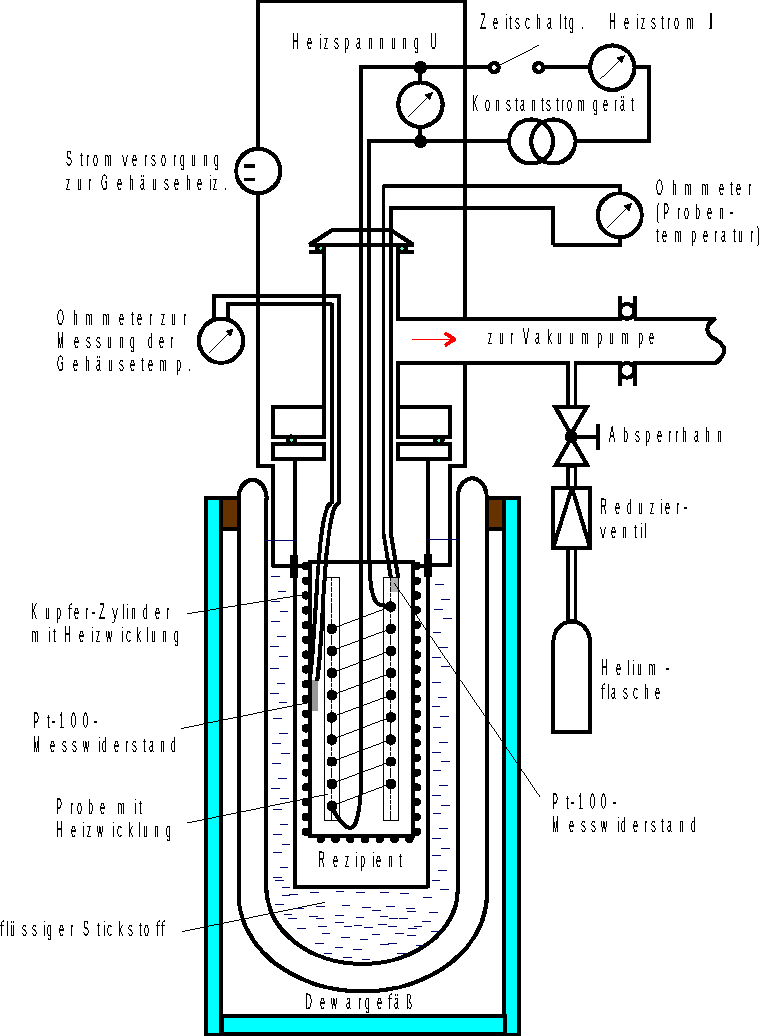
\includegraphics[scale=0.65]{Aufbau.pdf}
    \caption{Setup of the experiment \cite{V47}.}
    \label{fig:aufbau}
\end{figure}
The experimental setup for determining the specific heat of copper is housed in a Dewar flask filled with liquid nitrogen to ensure the 
required temperature range for this experiment. Inside the Dewar flask is the copper sample, which is surrounded by heating coils. The 
energy added by the heating coils to the sample and the temperature profile of the sample are measured during the experiment. The energy 
input is measured using the voltage and current with which the heating coils are operated, along with the time interval between two measurement 
points. The temperature of the sample is measured using the resistance of a PT-100 probe. To prevent heat losses through convection and heat 
conduction, a chamber enclosing the sample is evacuated for the measurement. Furthermore, a copper cylinder is positioned around the sample, 
which is ideally heated to the same temperature using another heating mantle to minimize radiative losses. The aforementioned quantities are 
measured at specific temperatures ranging from $80$ to $\SI{300}{\kelvin}$.
